%! Author = nico
%! Date = 23
\documentclass[a4paper, landscape, 8pt]{scrartcl}
\usepackage{csquotes}
\usepackage{subfiles}

% import template
% use german language
\usepackage[T1]{fontenc}
\usepackage[utf8]{inputenc}
\usepackage[english, ngerman]{babel}
\usepackage{lmodern}

% format
\usepackage{geometry}
\geometry{top=1.2cm, left=0.4cm, right=0.4cm}
\textheight = 550pt

% author
\usepackage{authblk}

% tables / tabular
\usepackage{tabularx}
\usepackage{makecell}
\usepackage{colortbl}

% math
\usepackage{amsmath}
\usepackage{amssymb}
\usepackage{amsfonts}
\usepackage{enumitem}

% graphic
\usepackage{graphicx}

% multi column
\usepackage{multicol}

%compact items
\setlist{topsep=0pt, leftmargin=4mm, nolistsep}
\setlength{\parindent}{0cm}

% header and footer
\usepackage{fancyhdr}
\pagestyle{fancy}

% header
\fancyhead[RO]{\AUTHOR | \INSTITUTE}
\fancyhead[LO]{\TITLE}

% footer
\fancyfoot[RO]{\CREATED}

\renewcommand\headrulewidth{0pt}
\renewcommand\footrulewidth{0pt}
\headsep = -2pt
\footskip = 0pt

% define Section format
\usepackage{sectsty}
\usepackage{titlesec}
\usepackage[dvipsnames]{xcolor}

\titleformat{name=\section}[block]{\sffamily\normalsize}{}{0pt}{\colorsection}
\titlespacing*{\section}{0pt}{0pt}{0pt}
\newcommand{\colorsection}[1]{%
	\colorbox{sectioncolor!80}{\parbox{0.98\linewidth}{\vspace{-1pt}\color{white}\ #1 \vspace{-2pt}}}}

% define Subsection format
\titleformat{name=\subsection}[block]{\sffamily\small}{}{0pt}{\colorsubsection}
\titlespacing*{\subsection}{0pt}{0pt}{0pt}
\newcommand{\colorsubsection}[1]{%
	\colorbox{subsectioncolor!80}{\parbox{0.98\linewidth}{\vspace{-1pt}\color{white}\ #1 \vspace{-2pt}}}}

% define SubSubsection format
\titleformat{name=\subsubsection}[block]{\sffamily\small}{}{0pt}{\colorsubsubsection}
\titlespacing*{\subsubsection}{0pt}{0pt}{0pt}
\newcommand{\colorsubsubsection}[1]{%
	\colorbox{subsubsectioncolor!60}{\parbox{0.98\linewidth}{\vspace{-1pt}\color{white}\ #1 \vspace{-2pt}}}}


% define colors
\definecolor{sectioncolor}{HTML}{191919}
\definecolor{subsectioncolor}{HTML}{0C5932}
\definecolor{subsubsectioncolor}{HTML}{0E693B}

\definecolor{b}{RGB}{0, 115, 192 } %Default highlight color
\definecolor{p}{RGB}{0, 43, 54} %Dark page color
\definecolor{t}{RGB}{131, 148, 150} %Dark text color

\definecolor{darkgreen}{RGB}{0,150,0}
\definecolor{dkgreen}{rgb}{0,0.6,0}
\definecolor{gray}{rgb}{0.5,0.5,0.5}
\definecolor{mauve}{rgb}{0.58,0,0.82}
\definecolor{DarkPurple}{rgb}{0.4, 0.1, 0.4}
\definecolor{DarkCyan}{rgb}{0.0, 0.5, 0.4}
\definecolor{LightLime}{rgb}{0.3, 0.5, 0.4}
\definecolor{Blue}{rgb}{0.0, 0.0, 1.0}
\definecolor{h}{RGB}{1, 101, 163}

% code listings
\usepackage{listings}
\usepackage{color}
\usepackage{beramono}
\usepackage{hyperref}
\hypersetup{
    colorlinks,
    linkcolor={black},
    citecolor={blue!50!black},
    urlcolor={blue!80!black}
}

\definecolor{bluekeywords}{rgb}{0,0,1}
\definecolor{greencomments}{rgb}{0,0.5,0}
\definecolor{redstrings}{rgb}{0.64,0.08,0.08}
\definecolor{xmlcomments}{rgb}{0.5,0.5,0.5}
\definecolor{types}{rgb}{0.17,0.57,0.68}

\definecolor{lstborder}{RGB}{24, 71, 21}
\definecolor{lstbackground}{RGB}{222, 230, 230}

\lstdefinestyle{eclipse-style}{
	frame=single,
	rulecolor=\color{lstborder},
	%backgroundcolor=\color{lstbackground},
	language=Java,
	showstringspaces=false,
	basicstyle=\ttfamily\scriptsize,
	keywordstyle=\color{RoyalBlue}\ttfamily,
    stringstyle=\color{darkgreen}\ttfamily,
	commentstyle=\color{DarkPurple!60}\ttfamily,
	identifierstyle=\color{black}\ttfamily,
	escapeinside={£}{£}, % latex scope within code
	breaklines=true,
	breakatwhitespace=true,
	showspaces=false,
	showtabs=false,
	tabsize=2,
	morekeywords={length},
	numberstyle=\tiny\color{darkgreen},
	aboveskip = 0em,
	belowskip = 0em,
	xleftmargin= 0em,
	framexleftmargin= 0em,
	gobble=20
}
\lstset{
	style=eclipse-style
	% literate=  % Allow for German characters in lstlistings.
	% {Ö}{{\"O}}1
	% {Ä}{{\"A}}1
	% {Ü}{{\"U}}1
	% {ü}{{\"u}}1
	% {ä}{{\"a}}1
	% {ö}{{\"o}}1}
}

% creation date
\usepackage{filemod}
\newcommand{\CREATED}{\filemodprintdate{\jobname}}

% front page
\newcommand{\AUTHOR}{Nico Fehr }
\newcommand{\INSTITUTE}{Ostschweizer Fachhochschule}

% no indentation
\setlength{\parindent}{0cm}

% new item tabitem for bullet points in tables
\newcommand{\tabitem}{~~\llap{\textbullet}~~}

\usepackage[ngerman]{babel}


% document information
\newcommand{\SUBJECT}{}
\newcommand{\TITLE}{Cheat sheet für Data Engineering (DatEng)}

% document content
\begin{document}

    \begin{multicols*}{4}
        \setlength{\columnseprule}{0.4pt}
        \footnotesize

        \section{Objekt-Relationale Mapper (O/R-Mapper)}
        Ziel: Semantische Lücke schliessen.
        Programme sind meist objektorientiert, DBs meist relational.

        \subsection{OR-Mapping Varianten}
        \begin{enumerate}
            \item Forward Engineering (Code first, Top-Down)
            \item Bottom Up (DB first, \enquote{Reverse Engineering})
            \item Inside-Out (Mapping first)
            \item Meet-in-the-middle (Outside-in)
            \item Meta Model (Model-driven)
        \end{enumerate}

        \subsection{JPA Layers}
        \begin{tabular}{l | l}
            \cellcolor{darkgreen!25} Java Program & Appl. mit persistenten Objekten \\
            \hline
            \cellcolor{Blue!25} JPA (Core) & Standard ORM Interface (JEE) \\
            \hline
            \cellcolor{darkgreen!25} JPA Provider & JPA Implementierung (Third Party) \\
            \hline
            \cellcolor{Blue!25} JDBC API & Standard JDBC Interface \\
            \hline
            \cellcolor{darkgreen!25} JDBC Driver & JDBC Driver (Third Party) \\
            \hline
            \cellcolor{gray!25} Database &
        \end{tabular}

        \subsection{Entity-Klassen}
        Können:
        \begin{itemize}
            \item erben, vererben
            \item interfaces implementieren
            \item abstract sein
        \end{itemize}
        Beispiel:
        \begin{lstlisting}[language=java]
                    @Entity
                    @Table(name = "account")
                    public class BankAccount {
                        @Id
                        @Column(name = "accountId")
                        private long id;

                        private double balance;

                        @Column(name = "salary", scale=10, precision=2)
                        private BigDecimal salary;

                        @Column(name = "description", length=500)
                        private String explanation;

                        @Temporal(TemporalType.TIMESTAMP)
                        private Calendar creationDate;

                        @Column(name = "s_time", columnDefinition="TIMESTAMPZ")
                        private Calendar startDate;

                        @Enumerated(EnumType.STRING)
                        private Currency curr;

                        @Column(name = "ssn", unique=true, nullable=true)
                        private long ssn;

                        @Transient
                        private String tempComments;

                        // getter und setter
                    }
        \end{lstlisting}

        Access Type von Annotations:
        \begin{tabularx}{\columnwidth}{X | X}
            Field Access & Property Access \\
            DB-Attr direkt in Fields abbilden (Spring default) & DB-Attr über Getter/Setter \\
            Nach Field-Annotation folgt Java-Feld & Nach Field-Annotation folgt Methode \\
            Von Spring bevorzugt &
        \end{tabularx}

        \subsection{Laden/Suchen von Entities}
        \begin{lstlisting}[language=java]
                    EntityManagerFactory factory = Persistence.createEntityManagerFactory("Bank");
                    EntityManager em = factory.createEntityManager();
                    Query query = em.createQuery("SELECT a FROM BankAccount a");
                    List<BankAccount> list = query.getResultList();
                    for (BankAccount account : list) {
                        System.out.println(account);
                    }
                    em.close();
        \end{lstlisting}

        \subsection{Insert von Entities \tiny{Explizit}}
        \begin{lstlisting}[language=java]
                    EntityManager em = factory.createEntityManager();
                    em.getTransaction().begin();
                    BankAccount account = new BankAccount();
                    account.setName("Bill");
                    em.persist(account);
                    em.getTransaction().commit();
                    em.close();
        \end{lstlisting}

        \subsection{Updates / Delete von Entities}
        \begin{lstlisting}[language=java]
                    EntityManager em = factory.createEntityManager();
                    em.getTransaction().begin();
                    BankAccount account = em.find(BankAccount.class, 1L);

                    // Update
                        account.incBalance(100);

                    // Delete
                        em.remove(account);
                    em.getTransaction().commit();
        \end{lstlisting}

        \subsubsection{Mapping in XML}
        Priorität Mapping
        \begin{enumerate}
            \item Mapping-File \enquote{orm.xml}
            \item Entity Annotationen
            \item Default Mapping (in JPA-Implementation)
        \end{enumerate}
        Beispiel:
        \begin{lstlisting}[language=xml]
                    <?xml version="1.0" encoding="UTF-8"?>
                    <entity-mappings version="1.0"
                      xmlns="http://java.sun.com/xml/ns/persistence/orm"
                      xmlns:xsi="http://www.w3.org/2001/XMLSchema-instance"
                      xsi:schemaLocation="http://java.sun.com/xml/ns/persistence/orm/orm_1_0.xsd">
                      <entity name="bankaccount" class="ch.hsr.dbs1.BankAccount" access="FIELD">
                       <table name="account"/>
                       <attributes>
                        <id name="id">
                            <column name="accountid"/>
                        </id>
                       </attributes>
                      </entity>
                    </entity-mappings>
        \end{lstlisting}

        \subsection{JPA Lifecycle}
        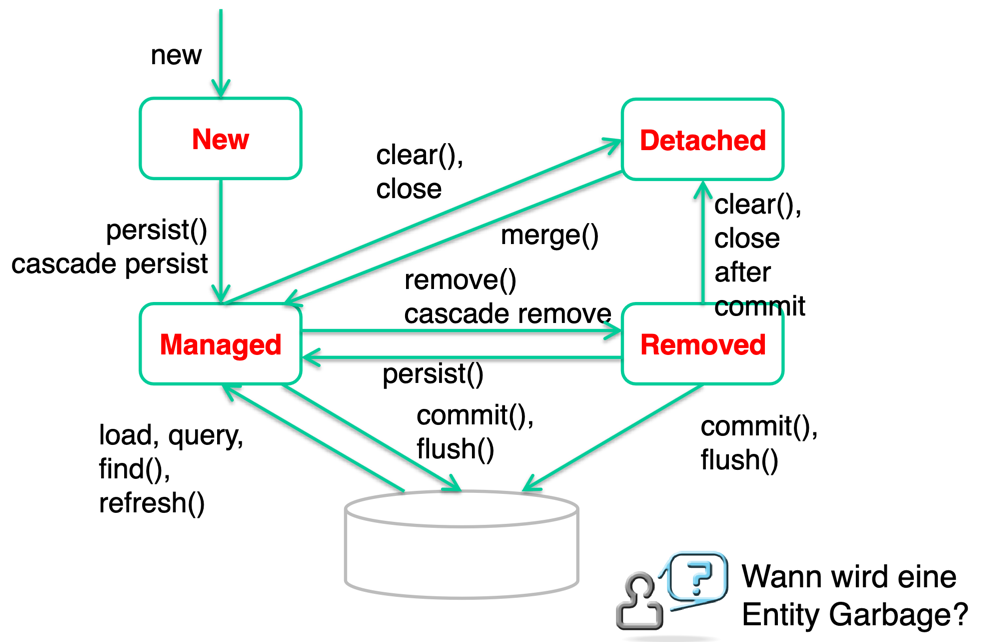
\includegraphics[scale=0.15]{graphic/00-entity-lifecycle}

        \subsection{JPA Architektur}
        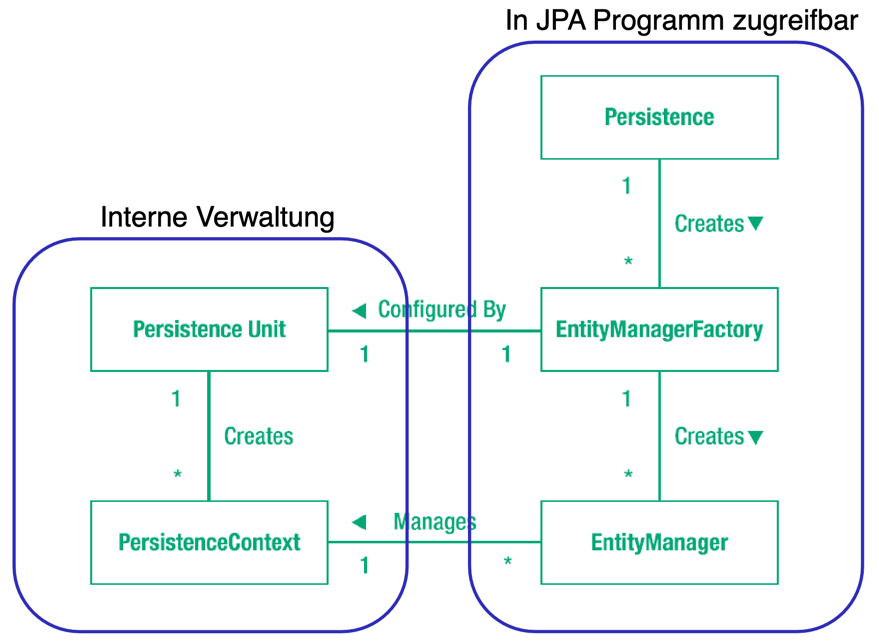
\includegraphics[scale=0.15]{graphic/01-jpa-architecture}

        \subsection{Entity States}
        Entitätsinstanzen befinden sich in einem von 4 Zuständen: \\
        \begin{tabularx}{\columnwidth}{l | X}
            New & keine persistente Identität, sind noch nicht mit Persistenzkontext verbunden\\
            \hline
            Managed & Entitätsinstanzen haben persistente Identität und sind mit Kontext verknüpft\\
            \hline
            Detached & Losgelöste Entitätsinstanzen haben Identität und sind derzeit nicht mit Kontext verbunden\\
            \hline
            Removed & Entfernte Instanzen haben Identität, sind mit Kontext verknüpft und sind für Entfernung aus Datenspeicher vorgesehen
        \end{tabularx}

        \subsection{JPA Transaktionen}

        \subsubsection{Transaction Isolation}

        \subsubsection{Optimistic Concurrency}

        \subsection{Lock Modes}
        \subsubsection{OPTIMISTIC}
        \subsubsection{OPTIMISTIC\_FORCE\_INCREMENT}

        \subsection{Object Identity}
        \begin{itemize}
            \item Session (=Instanz EntityManager, =Persistence Context) übersetzt DB Konzept von Primärschlüssel in Konzept von Objekt-Instanzen
            \item Session verwaltet Objekt Identität
            \subitem Objekte über Id im Cache verwaltet
            \subitem Bei 1. Zugriff wird Objekt aus DB geladen, bei weiteren, Kopie aus dem Cache
            \subitem Persistente Objekte identifiziert über DB-Identität
        \end{itemize}

        \subsubsection{Entity-Identität}
        \begin{itemize}
            \item Annotation @Id
            \item Generierung der Identity mit @GeneratedValue
            \item Verschiedene Strategien
            \subitem AUTO: von JPA Provider gewählt (meist SEQUENCE, IDENTITY)
            \subitem IDENTITY: basiert auf \enquote{auto-increment} (GENERATED AS...) Wert der DB
            \subitem SEQUENCE: basiert auf SEQUENCE DB-Objekt
            \subitem TABLE: basiert auf explizierter Primary-Key DB-Tabelle (selten)
        \end{itemize}

        \subsection{Generierungstypen}
        \subsubsection{Identity}
        \begin{lstlisting}[language=java]
                    @Id
                    @GeneratedValue(strategy = GenerationType.IDENTITY)
                    private long accountId;
        \end{lstlisting}
        \begin{lstlisting}[language=sql]
                    CREATE TABLE bankaccount (
                        accountid GENERATED ALWAYS AS IDENTY NOT NULL, -- frueher SERIAL in PostgreSQL
                        CONSTRAINT account_pkey PRIMARY KEY (accountid)
                        ...
                    )
        \end{lstlisting}

        \subsubsection{Sequence}
        \begin{lstlisting}[language=java]
                    @Id
                    @GeneratedValue(strategy = GenerationType.SEQUENCE, generator = "BankCustGen")
                    @SequenceGenerator(name = "BankCustGen",
                                       sequenceName = "customeridseq",
                                       allocationSize = 1)
                    // nur einmal ausfuehren
                    private long customerId;
        \end{lstlisting}
        \begin{lstlisting}[language=sql]
                    -- explizites sequence Objekt in DB
                    CREATE SEQUENCE customeridseq;
        \end{lstlisting}

        \subsubsection{Table}
        \begin{lstlisting}[language=java]
                    @Id
                    @GeneratedValue(strategy = GenerationType.TABLE,
                        generator = "CustomerGen")
                    @TableGenerator(name = "CustomerGen", table = "keytable",
                        pkColumnName = "keyname",
                        valueColumnName = "keyvalue",
                        pkColumnValue = "customerkey")
                    private long customerId;
        \end{lstlisting}

        \textbf{keytable} (Tabelle zur Key-Verwaltung)\\
        \begin{tabularx}{\columnwidth}{l | X}
            \textbf{keyname} & \textbf{keyvalue} \\
            \hline
            customerkey & 100 \\
            \hline
            accountkey & 3214
        \end{tabularx}

        \subsection{Bidirektionalität}
        \subsubsection{Inkonsistenz}
        Bidirektionale Relationen sind bei Änderungen durch JPA nicht synchronisiert.
        \begin{itemize}
            \item Trotz Angabe von \texttt{@OneToMany(mappedBy="customer")}
            \item Nur nach Laden konsistent
        \end{itemize}

        \subsection{Kardinalitäten}
        \subsubsection{OneToOne (1:1)}
        Insert image

        \subsubsection{ManyToOne (Many:1)}
        Insert image

        \subsubsection{OneToMany (1:Many)}
        \subsubsection{ManyToMany (Many:Many)}


        \subsubsection{Bidirectional Sync}

        \subsection{Vererbung: Abbildungsstrategien}
        \begin{tabularx}{\columnwidth}{l | X}
            SINGLE TABLE & Einzige Tabelle für Superklasse (+ type); JPA Default. (3c) \\
            \hline
            JOINED TABLE & Je Tabelle pro Sub- und Superklasse (+ type + Beziehungen). (3a, \enquote{Tabelle pro Klasse}) \\
            \hline
            TABLE PER CLASS & Je Tabelle pro Klasse (inkl. vererbte Columns), d.h. mit redundanten Columns (3b, hatte keine Superklasse) \\
            \hline
            MAPPED SUPERCLASS & Je Tabelle pro Klasse (inkl. vererbte Columns). Ähnlich wie TABLE PER CLASS aber ohne Superklasse. (3b)
        \end{tabularx}

        \subsubsection{Single Table}

        \subsubsection{Joined Table}
        \subsubsection{Table per Class}
        \subsubsection{Mapped Superclass}

        \section{JPQL \tiny{Java Persistence Query Language}}
        \subsection{Query Parameters}
        \begin{tabularx}{\columnwidth}{l | X}
            Positional & \texttt{select a from BankAccount a where a.customer.name like \textcolor{red}{?1} and a.balance >= \textcolor{red}{?2}} \\
            \hline
            Named & \texttt{select a from BankAccount a where a.customer.name like \textcolor{red}{:name} and a.balance >= \textcolor{red}{:lower}}
        \end{tabularx}

        \subsection{Criteria API}

        \subsection{Weitere Beispiele}


        \section{Stored Procedures}
        Synonyme: User Defined Functions, Subroutine, Methode.

        \begin{tabularx}{\columnwidth}{l | X}
            Vorteile & \tabitem Domänen Logik (Funktionen, Datenkapselung) \\
            & \tabitem Performanz: Funktionen nahe bei Daten \\
            & \tabitem Triggers \\
            & \tabitem Konsistenz: Triggers Security (GRANT auf SP, Log auditing) \\
            & \tabitem Separation of Concern/Duties sowie Wiederverwendbarkeit des Codes \\
            \hline
            Nachteile & \tabitem Manchmal reichen Views \\
            & \tabitem Manchmal reichen ORM (Object-Relational Mapper) \\
            & \tabitem Macht Software-Entwicklungsprozess komplizierter \\
            & \tabitem Portierbarkeit
        \end{tabularx}

        \subsection{Syntax}
        \begin{lstlisting}[language=sql]
                    create [or replace] [function | procedure] name ( [ [argname] argtype [,...] ] )
                        [ returns rettype | returns setof record ]
                    language [plpgsql | SQL | ...] [optimizers]
                    as $$
                      -- ... Source Code gemaess "language"
                    $$;

                    drop function name(argtype [,...]);
        \end{lstlisting}

        \section{PL/pgSQL \tiny{Prozedurale Sprache von PostgreSQL}}
        Hello World: \\
        \begin{lstlisting}[language=sql]
                    -- Hello World
                    create or replace function helloworld()
                    returns void language plpgsql as $$
                    begin
                       raise notice 'Hello World!';
                    end;
                    $$;

                    -- Test and use the function/procedure:
                    select helloworld();
        \end{lstlisting}

        PL/pgSQL mit Paramter: \\
        \begin{lstlisting}[language=sql]
                    create or replace function
                      pow_mod(bigx bigint, n bigint, m bigint)
                    returns bigint as $$
                    declare
                      x bigint;
                      xx bigint;
                    begin
                      if n = 0 then return 1; end if;
                      x := bigx % m;
                      xx := (x * x) % m;
                      if n % 2 = 0 then
                        return pow_mod(xx, n/2, m);
                      else
                        return (x * pow_mod(xx, (n-1)/2, m)) % m;
                      end if;
                    end;
                    $$ language plpgsql;
        \end{lstlisting}

        \subsection{SP Compiler}
        \begin{enumerate}
            \item Code wird beim Aufruf geparsed
            \item als Pseudocode in der DB gespeichert
            \item bei der ersten Ausführung wird volle Syntax gecheckt
            \item SQLStatements werden vorkompiliert (wie JDBC PreparedStatement) und bei wiederholtem Aufruf wiederverwendet.
            \item Code läuft im Server ab
            \item Kommunikation mit Frontend über Rückgabewerte (SP ungeeignet für GUI)
        \end{enumerate}s

        \section{Triggers}
        \begin{itemize}
            \item Implementation von komplexen Konsistenzbedingungen
            \item Sicherheit, z.B. wenn Änderungen nur während Arbeitstagen ausgeführt werden können
            \item Berechnen von abgeleiteten Attributen
            \item Sammlen von Statistik- und Logdaten
            \item DB-Objekte $\to$ immer einer Tabelle zugeordnet
            \item in SP programmiert, namentlich als PL/pgSQL-Function
            \item haben keine Funktions-Parameter
            \item können nicht direkt aufgerufen werden
            \item werden vom DBMS beim Eintreten eines \enquote{DB-Events} aufgerufen
            \item haben bei Ausführung die Rechte ihres Owners
        \end{itemize}

        \subsection{Syntax}

        \subsection{Trigger-Funktions-Variablen}
        \begin{tabularx}{\columnwidth}{l | X}
            \textbf{TG\_NAME} & Name von Trigger \\
            \textbf{TG\_WHEN} & BEFORE / AFTER \\
            \textbf{TG\_LEVEL} & ROW / STATEMENT \\
            \textbf{TG\_OP} & INSERT, UPDATE, DELETE, TRUNCATE \\
            \textbf{TG\_RELID} & ROW ID der Tabelle \\
            \textbf{TG\_RELNAME} & Name der Tabelle \\
            \textbf{TG\_TABLE\_SCHEMA} & Schema der Tabelle \\
            \textbf{NEW, OLD} & neue / alte Records
        \end{tabularx}

        \subsection{Auditing mit Triggers}
        \begin{lstlisting}[language=sql]
                    CREATE TABLE ang_audit(
                        operation char(1)   NOT NULL,
                        stamp timestamp NOT NULL,
                        userid text      NOT NULL,
                        angname text      NOT NULL,
                        salaer integer
                    );

                    CREATE TRIGGER ang_audit
                    AFTER INSERT OR UPDATE OR DELETE ON Angestellter
                    FOR EACH ROW
                    EXECUTE PROCEDURE process_ang_audit();

                    CREATE OR REPLACE FUNCTION process_ang_audit()
                    RETURNS TRIGGER AS $$
                        BEGIN
                            IF (TG_OP = 'DELETE') THEN
                                INSERT INTO ang_audit
                                SELECT 'D', now(), user, OLD.name, OLD.salaer;
                                RETURN OLD;
                            ELSIF (TG_OP = 'UPDATE') THEN
                                INSERT INTO ang_audit
                                SELECT 'U', now(), user, NEW.name, NEW.salaer;
                            ELSIF (TG_OP = 'INSERT') THEN
                                INSERT INTO ang_audit
                                SELECT 'I', now(), user, NEW.name, NEW.salaer;
                            END IF;
                            RETURN NULL; -- result ignored => AFTER trigger
                        END;
                    $$ language plpgsql;
        \end{lstlisting}

        \subsection{Ausschalten}
        \begin{lstlisting}[language=sql]
                    ALTER TABLE mytable DISABLE TRIGGER mytrigger | ALL;
        \end{lstlisting}

        \section{Updatable Views}
        \begin{lstlisting}[language=sql]
                    CREATE VIEW myview AS SELECT ...
        \end{lstlisting}
        Updatable Views erstellen mit:
        \begin{itemize}
            \item Stored Procedures
            \item Updatable Views - automatisch aktualisierbare Views
            \subitem automatisch aktualisierbare Views
            \subitem nur möglich, wenn bestimmte Bedingungen erfüllt
            \item Instead of-Triggers
        \end{itemize}

        Views sind automatisch aktualisierbar wenn:
        \begin{itemize}
            \item Genau einen Eintrag in der FROM-Klausel (andere Tabelle oder andere updatable View)
            \item Keine WITH, DISTINCT, GROUP BY, HAVING, LIMIT, OFFSET
            \item kein UNION, INTERSECT, EXCEPT
            \item SELECT-Liste besitzt keine Aggregation, Window-Funktion oder SET-Returning-Funktion
        \end{itemize}

        \subsection{Instead of-Triggers}
        Nur für Views und nicht für Tabelle möglich.
        Leiten Modifikation (INSERT, UPDATE, DELETE) auf Views zur darunterliegenden Tabelle weiter.

        \begin{lstlisting}[language=sql]
                    --DROP FUNCTION IF EXISTS abtleiterinfo_update_abtchef_fn() CASCADE;
                    CREATE OR REPLACE FUNCTION abtleiterinfo_update_abtchef_fn()
                    RETURNS TRIGGER AS $$
                        BEGIN
                            IF TG_OP = 'UPDATE' THEN
                                UPDATE abtleitung SET abtchef=NEW.abtchef WHERE abtnr=OLD.abtnr;
                                RETURN NEW; -- New Record ist resultset
                            END IF;
                        END;
                    $$ LANGUAGE plpgsql;

                    CREATE TRIGGER abtleiterinfo_update_abtchef
                        INSTEAD OF UPDATE ON abtleiterinfo
                        FOR EACH ROW
                        EXECUTE PROCEDURE abtleiterinfo_update_abtchef_fn();

                    UPDATE abtleiterinfo SET abtchef=1019 WHERE abtnr=2; -- is possible now
        \end{lstlisting}

        \section{Materialized Views}
        \begin{lstlisting}[language=sql]
                    -- create materialized view (snapshot)
                    CREATE MATERIALIZED VIEW myMatView as SELECT ...

                    -- refresh materialized view
                    REFRESH MATERIALIZED VIEW myMatView;

                    -- refresh materialized view concurrently (view is available during updates)
                    REFRESH MATERIALIZED VIEW CONCURRENTLY myMatView;
        \end{lstlisting}

        \begin{tabularx}{\columnwidth}{l X}
            Snapshot & updated once (REFRESH in PostgreSQL) \\
            \hline
            Eager & updates as underlying table is updated \\
            \hline
            Lazy & updated when transaction commits \\
            \hline
            Andere & Oracle: \enquote{User defined}, \enquote{Per Interval}
        \end{tabularx}

        \subsection{Temporäre Tabellen}
        Tabelle wird automatisch am Ende der Transaktion oder Session gelöscht.
        \begin{lstlisting}[language=sql]
                    CREATE TEMPORARY TABLE tmp AS SELECT ...
        \end{lstlisting}

        \section{Datentyp}
        \subsection{Abstrakter Datentyp {\tiny ADT}}
        Datentyp, der durch Operationen definiert ist, Zugriff und Verwaltung zu ermöglichen und realisieren.
        HINWEIS: ADT kann ADT enthalten, z.B. Stack als Liste.
        Bestandteile:
        \begin{tabularx}{\columnwidth}{l | X}
            \textbf{Datentyp ADT} & \textbf{Beispiel} \\
            \hline
            Name & \texttt{easteregg} \\
            Innere Datenstruktur & \texttt{outer: text, inner: text;} \\
            Konstruktor & \texttt{easteregg\_from\_text('x', 'yy')} \\
            Accessor-Funktion & \texttt{easteregg\_inner()} \\
            Update-Funktion & \texttt{easteregg\_append('zz')} \\
            Hilfs-Funktion & \texttt{easteregg\_astext(myegg)} \\
            Operator & \texttt{WHERE myegg = youregg} \\
            Index auf Attribut \texttt{eggs} & \texttt{CREATE INDEX myindex ON mytable USING GIN(eggs);}
        \end{tabularx}

        \subsection{User-Defined Datentypen in PostgreSQL}
        \begin{multicols*}{2}
            \textbf{CREATE DOMAIN ...}
            \begin{itemize}
                \item erstellt benutzerdefinierten Datentyp
                \item für Datenschema und SP
                \item mit Constraints wie NOT NULL, CHECK
            \end{itemize}
            \begin{lstlisting}[language=sql]
                    create domain contact_name as
                        varchar(255) not null
                            -- (!~) does not match (regex), case sensitive
                            check (value !~ '\s');
            \end{lstlisting}

            \columnbreak

            \textbf{CREATE TYPE ...}
            \begin{itemize}
                \item zusammengesetzter Datentyp
                \item für Datenschema und SP
                \item auch für ENUM Type
                \item Keine Constraints
            \end{itemize}
            \begin{lstlisting}[language=sql]
                    create type easteregg as (
                        outer: text,
                        inner: text,
                    );
                    create type traffic_light_t as
                        enum('red', 'yellow', 'green');
            \end{lstlisting}
        \end{multicols*}

        \section{Collections}
        \begin{itemize}
            \item Lineare Kollektionen
            \subitem Listen/Arrays - Priority Queues/Heaps
            \item Assoziative Kollektionen
            \subitem Sets, Bags/Multisets - Dictionaries (Associative Arrays)
            \item Graphen und Trees
        \end{itemize}

        \subsection{Arrays}
        Achtung: Arrays $\neq$ Sets.
        Sets $\to$ separate Tabelle (besonders bei vielen Updates).
        Arrays (fixe oder variable Länge) sind Erweiterung jedes Basisdatentyps (int, boolean, etc.).

        \begin{lstlisting}[language=sql]
                    CREATE TABLE sal_emp (
                        pay_by_quarter integer[] -- 1 dim.
                        schedule text[][] ); -- unbound 2 dim.
        \end{lstlisting}

        \begin{lstlisting}[language=sql]
            SELECT ARRAY[1.1, 2.1, 3.1]::int[] = ARRAY[1, 2, 3]; -- ergibt "t" für true
        \end{lstlisting}

        \subsection{Dictionaries}
        Schema-Less, für variable, unvorhersehbare, unkoordinierbare Werte
        Schlüssel-Werte-Paare, die einen Unique Key auf einen Value abbilden.
        Auch als Associative Array, Map Collection, Key-Value Pair (KVP), Hash, Object-Attribute-Values, Entity Attribute Value bekannt.

        \subsubsection{hstore}

        \subsection{Graphs}
        \subsection{Trees}
        
        \subsection{Semistrukturierte Daten {\tiny XML, JSON}}
        \subsubsection{JSON}

        \subsubsection{XML}


        \section{Database-as-a-service (DBAAS)}
        TODO

        \section{GraphQL}
        REST Alternative



        \section{Database Design Patterns}
        \subsection{Data Mapper}
        \begin{itemize}
            \item CRUD-Funktionen auf Objekten (in DB persistent)
            \item Bildet Entität in DB ab
            \item Implementiert durch OR/Mapper
        \end{itemize}

        \subsection{Active Record}
        \begin{itemize}
            \item Speichert Daten in relationaler Datenbank
            \item \enquote{One Object - One Record}
        \end{itemize}

        \subsection{CQRS {\tiny Command-Query Responsibility Segregation}}
        TODO

        \subsection{Event Sourcing}
        \enquote{Turning the database inside-out}
        TODO

        \subsection{Evolutionary Database Design}
        TODO

    \end{multicols*}
\end{document}